\documentclass{article}

\usepackage[english]{babel}

\usepackage[letterpaper,top=2cm,bottom=2cm,left=3cm,right=3cm,marginparwidth=1.75cm]{geometry}

\usepackage{amsmath}
\usepackage{graphicx}
\usepackage[colorlinks=true, allcolors=blue]{hyperref}

\title{Labwork 1}
\author{BA11-103 - Nguyen Quang Vinh}

\begin{document}
\maketitle

\section{Protocol}

\begin{figure}[h]
\centering
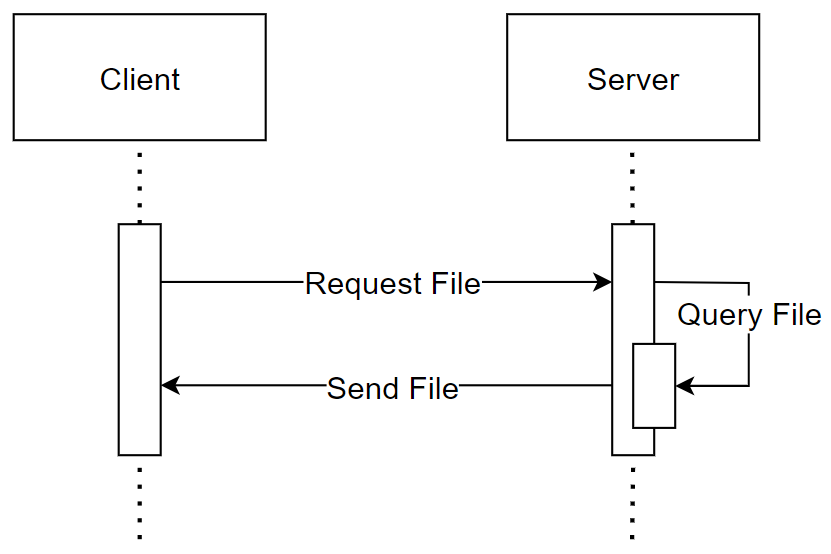
\includegraphics[width=0.8\linewidth]{Protocol.png}
\caption{\label{fig:Protocol}Protocol Design.}
\end{figure}

\section{System Organization}

\begin{figure}[h]
\centering
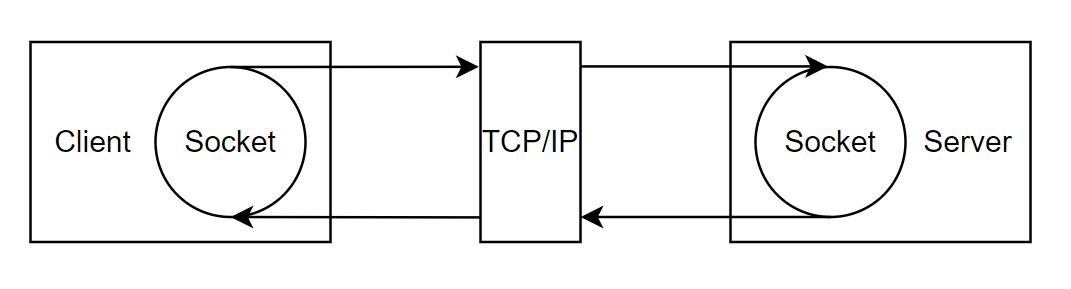
\includegraphics[width=0.8\linewidth]{System.png}
\caption{\label{fig:System}System architecture.}
\end{figure}

\section{File Transfer}
\subsection{Server Side (server.c)}
\begin{verbatim}
a. Preparation: It includes necessary files for network communication (sockets), standard 
input/output (stdio.h), and memory management (stdlib.h). A port number (PORT) is defined 
for listening on connections.
b. Socket Creation: The server creates a communication endpoint (socket) using `socket` 
specifying the internet protocol version (IPv4) and the reliable stream-based protocol (TCP).
c. Socket Configuration: It allows address and port reuse with `setsockopt` to avoid 
binding issues on restarts. The server then sets up its listening address structure:
    - Address family is set to IPv4 (AF_INET).
    - It listens on all available interfaces (`INADDR_ANY`).
    - The port is set to the defined `PORT` and converted to network byte order using `htons`.
d. Binding and Listening: The server binds the socket to the specified address and port 
using `bind`. Then, it starts listening for incoming client connections on the bound 
socket with a queue length of 3 using `listen`.
e. Accepting a Client: When a client connects, the server accepts the connection with 
`accept`, creating a new dedicated socket for communication with that specific client.
f. Receiving Filename: The server reads data from the client (potentially a greeting 
message) using `read` and stores it in a buffer. It then reads the actual filename
requested by the client and constructs the full path to the requested file.
g. Opening and Sending File: It opens the requested file in read mode and checks for 
successful opening. The server reads the file contents line by line using `fgets` and sends 
each line to the client using `send`.
h. Cleanup: After successful file transmission, the server closes the opened file and the 
client connection. Finally, it closes its own listening socket and exits the program. 
\end{verbatim}

\subsection{Client Side (client.c)}
\begin{verbatim}
a. Preparation: It includes necessary files for network communication (sockets), standard 
input/output (stdio.h), and string manipulation (string.h). A port number (PORT) is 
defined for connecting to the server.
b. Socket Creation: The client creates a communication endpoint (socket) using `socket` 
specifying the internet protocol version (IPv4) and the reliable stream-based protocol (TCP).
c. Server Address Setup: The client sets up the server's address information:
    - Address family is set to IPv4 (AF_INET).
    - Port is set to the defined `PORT` and converted to network byte order using `htons`.
    - It converts the loopback address "127.0.0.1" (referring to itself) into a binary 
    network address structure using `inet_pton`.
d. Connecting to Server: The client attempts to connect to the server at the specified 
address and port using `connect`.
e. Sending Filename Request: Upon successful connection, the client sends the filename 
"file.txt" to the server using `send`.
f. Receiving File Content: The client attempts to read data from the server using `read`. 
   - If an error occurs during reading, it exits with an error message.
   - If no data is received (`valread` is 0), it indicates the server might have closed 
   the connection.
   - Otherwise, it reads the received data (potentially the file content) and null-terminates 
   the string for proper printing. The content is then printed to the console.
g. Receiving Additional Message (Optional): The client reads again from the server 
using `read`. This part might be specific to the server implementation and could potentially 
receive an acknowledgement or additional information. The received data is printed 
to the console.
h. Cleanup: The client closes the connection to the server using `close` and exits the program. 
\end{verbatim}

\subsection{Communication}
Leveraging a TCP connection, a client-server data transfer takes place. The client reads data segments from a file and sends them to the server. The server receives these segments, reassembles them, and writes the complete data to a designated file on its local storage.

\end{document}